\documentclass[a4paper, 12pt]{extarticle}
\usepackage[dvipsnames]{xcolor}
\usepackage[top=70pt,bottom=70pt,left=48pt,right=46pt]{geometry}
\definecolor{header}{RGB}{252, 171, 16}
\definecolor{defenition}{RGB}{248, 51, 60}
\definecolor{main_title}{RGB}{43, 158, 179}
\definecolor{sub_header}{RGB}{68, 175, 105}
\usepackage[english, russian]{babel}
\usepackage[utf8]{inputenc}
\usepackage{amsmath}
\usepackage[most]{tcolorbox}
\usepackage{listings}
\usepackage{graphicx}
\usepackage{amsmath}
\usepackage{lettrine}
\title{\textcolor{main_title}{Фотоэлектрический способ преобразования энергии солнечного излучения}}

\author{% 
    {Абрамов Александр, Б04-104} \\
    {Алямовская Анна Андреевна, Б04-103}\\
    {Раводина Александра Михайловна, Б04-103} \\
    {Шмаков Владимир Евгеньевич, Б04-103}%
}

\newtcolorbox{fequation}[1][]{ams equation*,size=small,#1}








\begin{document}
\maketitle



\section*{\textcolor{header}{Цель работы}}

\begin{itemize}
    \item Исследование темновой и световой вольтамперных характеристик фотоэлемента.
    \item Изучение влияния мощности падающего излучения на характеристики образца с помощью фильтров.
\end{itemize}

\section*{\textcolor{header}{Теоретические сведения}}



\begin{figure}[htbp]
    \centering
    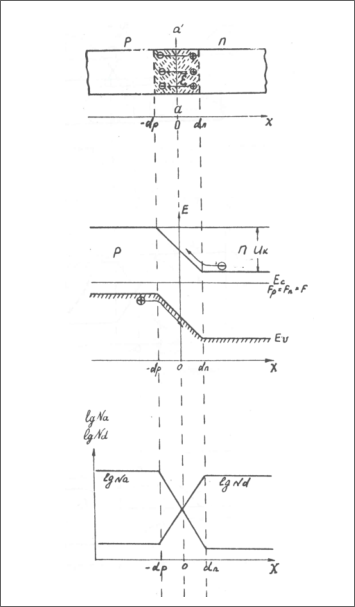
\includegraphics[width = 0.3\textwidth]{pics/diode.png}
    \caption{$p-n$ переход}
    \label{fig:diode}
\end{figure}


\lettrine{\textcolor{defenition}{П}}{\textcolor{defenition}{рямое преобразование}} лучистой энергии Солнца в электрическую осуществляется с помощью фотоэффекта на потенциальном барьере или так называемого вентильного фотоэффекта, суть которого – возникновение фото-ЭДС при освещении контактов металл-полупроводник и $p-n$ переходов. Однако, вследствие сложной микроструктуры контактов полупроводника с металлом, мы ограничимся в дальнейшем наиболее ясным случаем $p-n$  переходов.
Рассмотрим более подробно, что представляет собой  переход. Пусть два полупроводника, один из которых имеет проводимость p-типа, а другой n-типа
приводятся в хороший контакт по плоскости $a a'$, как показано на рисунке(\ref{fig:diode}). Тогда под действием градиента концентрации дырки из приконтактного слоя $p$ - области будут диффундировать в $n$-область, а электроны из приконтактного слоя $n$-области в $p$-область. В результате такой диффузии в приконтактном слое $p$-области создается отрицательный объемный заряд нескомпенсированных ионов акцепторной примеси, а в приконтактном слое $n$-области – положительный объемный заряд нескомпенсированных ионов донорной примеси. Порожденное объемными зарядами электрическое поле (направление которого показано на рисунке \ref{fig:diode}), будет препятствовать дальнейшей диффузии основных носителей зарядов (основными называются носители, знак которых соотвествует типу проводимости полупроводника). При этом напряженность электрического поля  и толщины слоев объемных зарядов в $n$ и $p$ -областях будут возрастать до тех пор, пока не достигнут своих равновесных значений $\epsilon_c$, $d_p$ и $d_n$, при которых диффузионные потоки основных носителей зарядов полностью скомпенсированы дрейфовыми потоками, вызванными электрическим полем объемных зарядов. 

Состояние $p-n$-перехода в термодинамическом равновесии легко понять, обращаясь к его энергетической диаграмме, приведенной на рисункe \ref{fig:diode}. Здесь  $E_c$– дно зоны проводимости,  $E_v$– потолок валентной зоны,  $F$– уровень Ферми. В самом деле, электроны из $n$-области не могут проникнуть в $p$-область, так как для этого им необходимо преодолеть потенциальный барьер, высота  которого равна контактной разности потенциалов, а энергия электронов меньше высоты этого барьера. По аналогичной причине дырки из $p$-области не могут попасть в $n$-область.


\section*{\textcolor{header}{Методика}}

\begin{figure}[htbp]
    \centering
    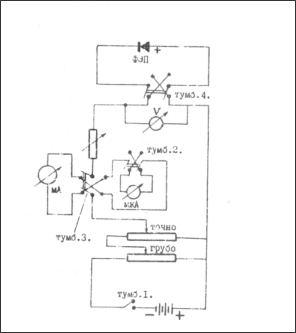
\includegraphics[width = 0.35\textwidth]{pics/setup.png}
    \caption{Схема экспериментальной установки}
    \label{fig:setup}
\end{figure}
\subsection*{\textcolor{sub_header}{Оборудование}}

\begin{itemize}
    \item Фотоэлектрический преобразователь
    \item Микроамперметр
    \item Миллиамперметр
    \item Вольтметр
    \item Блок питания
    \item Потенциометры
    \item Набор оптических фильтров
    \item Лампа 
\end{itemize}

\subsection*{\textcolor{sub_header}{Экспериментальная установка}}


Вольтамперная характеристики фотопреобразователя могут быть измерены с помощью схемы, представленной на рисункe \ref{fig:setup}. Когда преобразователь работает как генератор электроэнергии, то в качестве источника излучения используется лампа марки 3H7 или 3Н8 с встроенным зеркальным отражателем и мощностью 500 Вт. Спектр ее излучения с помощью водяного фильтра приближен к спектру солнечного излучения и к спектральной чувствительности кремниевого преобразователя.



\section*{\textcolor{header}{Обработка экспериментальных данных}}

\subsection*{\textcolor{sub_header}{Темновые характеристики}}
\begin{figure}[htbp]
    \centering
    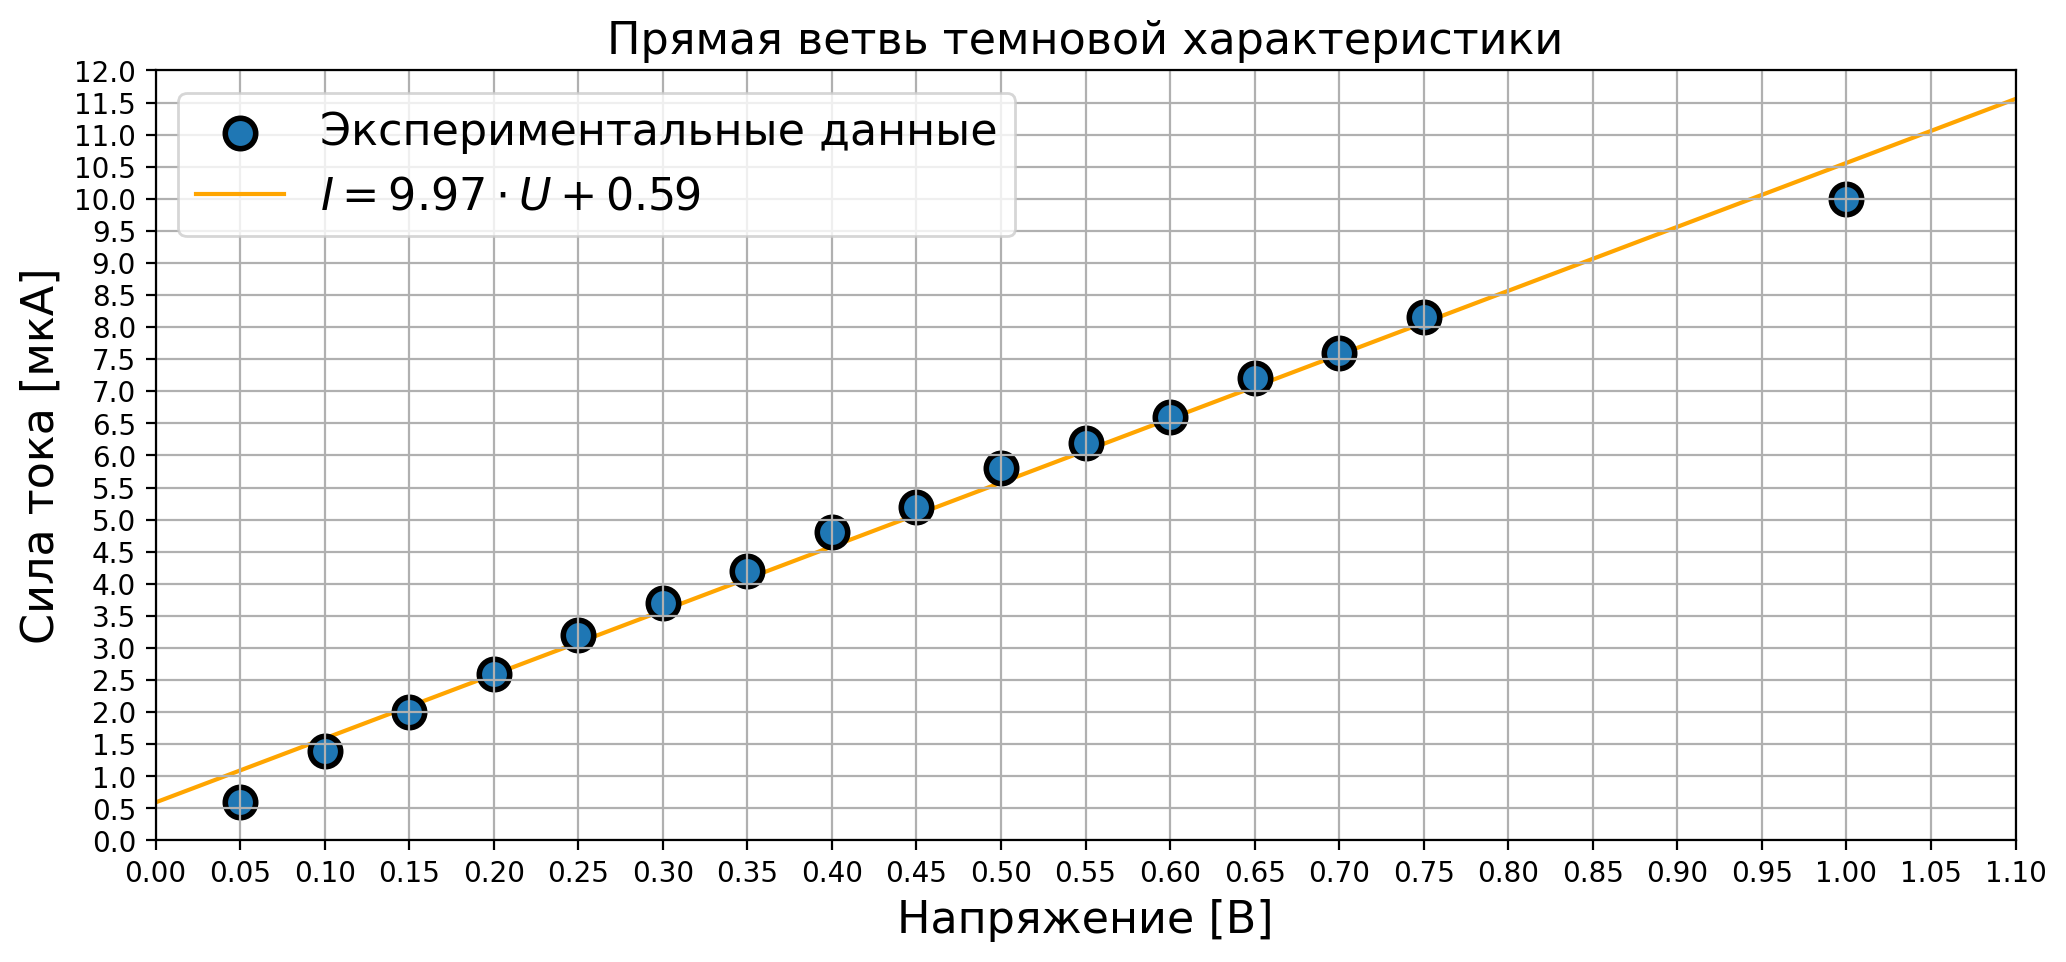
\includegraphics[width = 0.8\textwidth]{pics/dark_straight.png}
    \caption{Прямая ветвь темновой характеристики}
    \label{fig:dark_straight}
\end{figure}

Прямая ветвь темновой характеристики изображена на рисунке \ref{fig:dark_straight}. По наклону кривой посчитаем прямое сопротивление фотопреобразователя:
$$
R_{\text{пр}} = \frac{d U_{\text{пр}}}{d I_{\text{пр}}} = \frac{1}{a} \sim 100 \text{кОм}
$$

Обратная ветвь темновой характеристики изображена на рисунке \ref{fig:dark_back}.
$$
R_{\text{обр}} = \frac{d U_{\text{обр}}}{d I_{\text{обр}}} = \frac{1}{a} \sim 41 \text{кОм} 
$$

\begin{figure}[htbp]
    \centering
    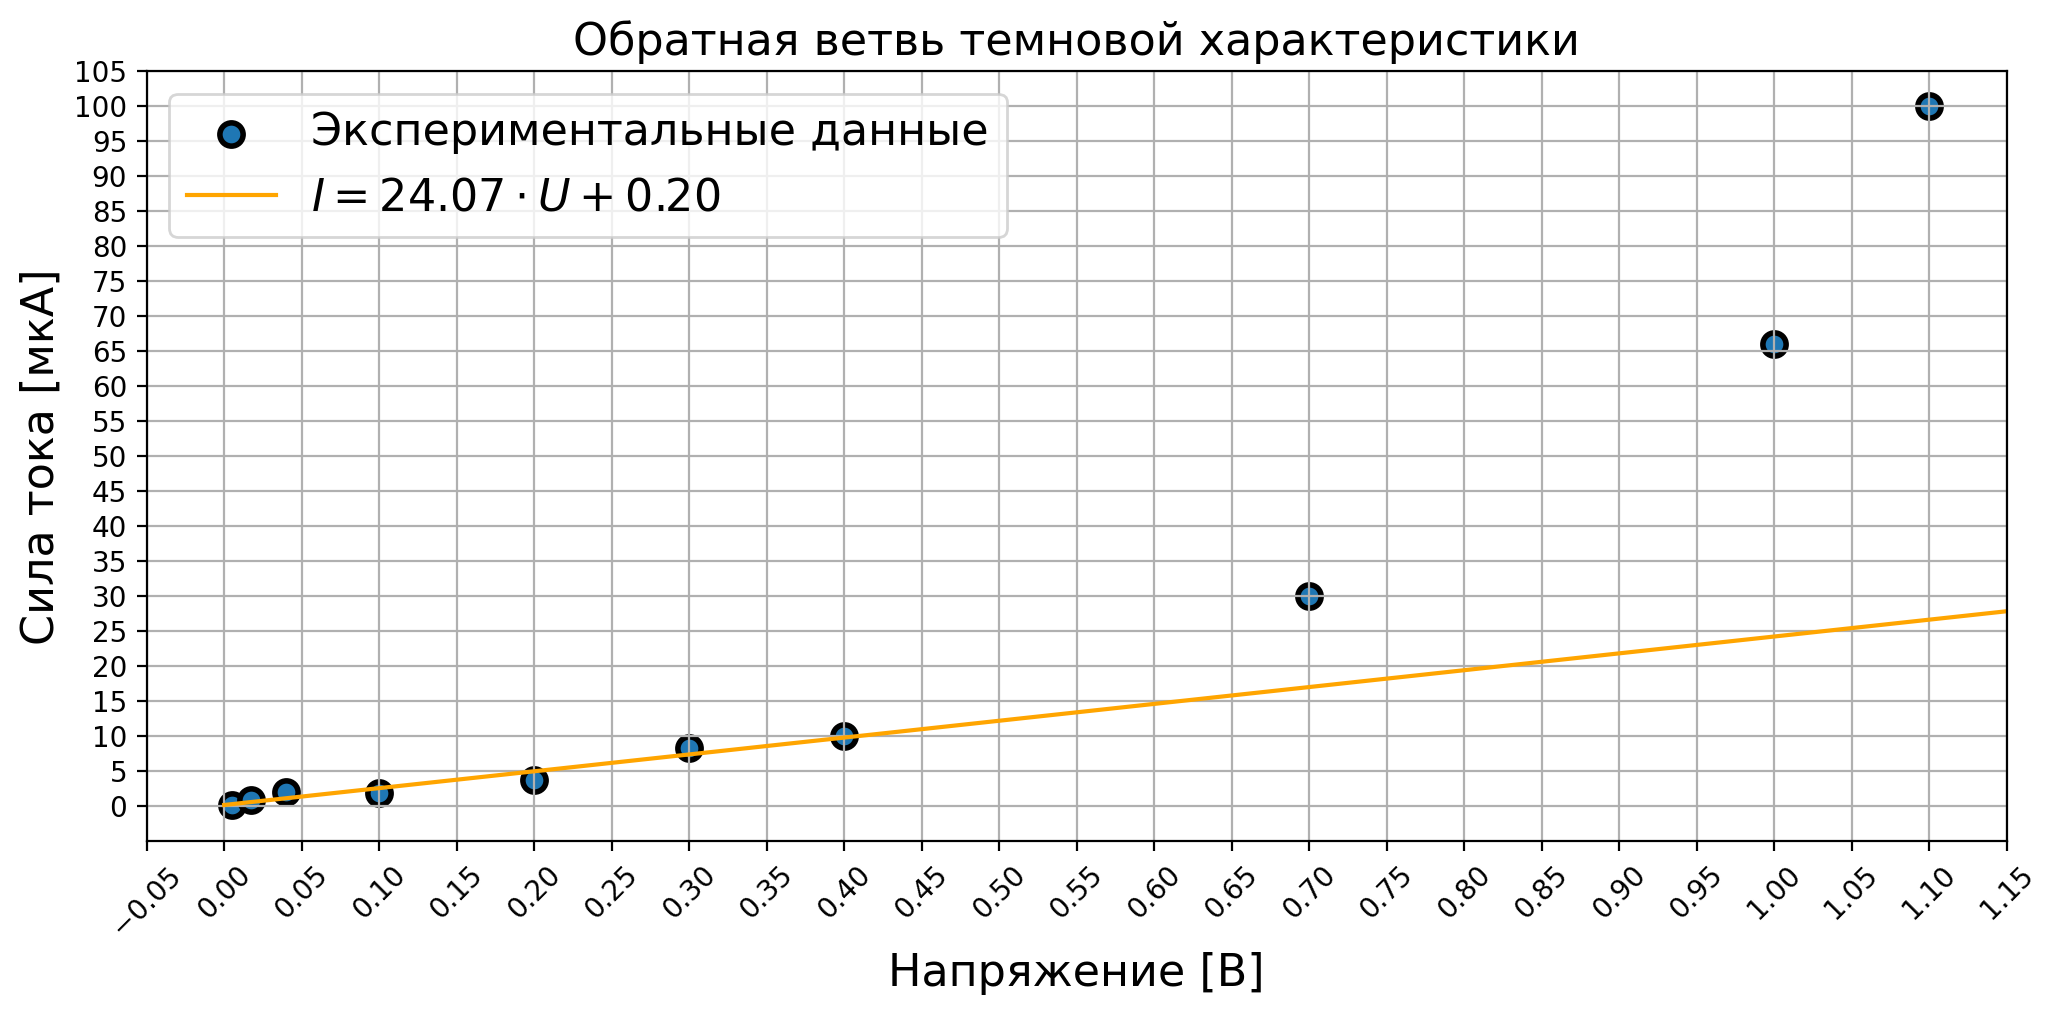
\includegraphics[width = 0.8\textwidth]{pics/dark_back.png}
    \caption{Обратная ветвь темновой характеристики}
    \label{fig:dark_back}
\end{figure}


\begin{figure}[htbp]
    \centering
    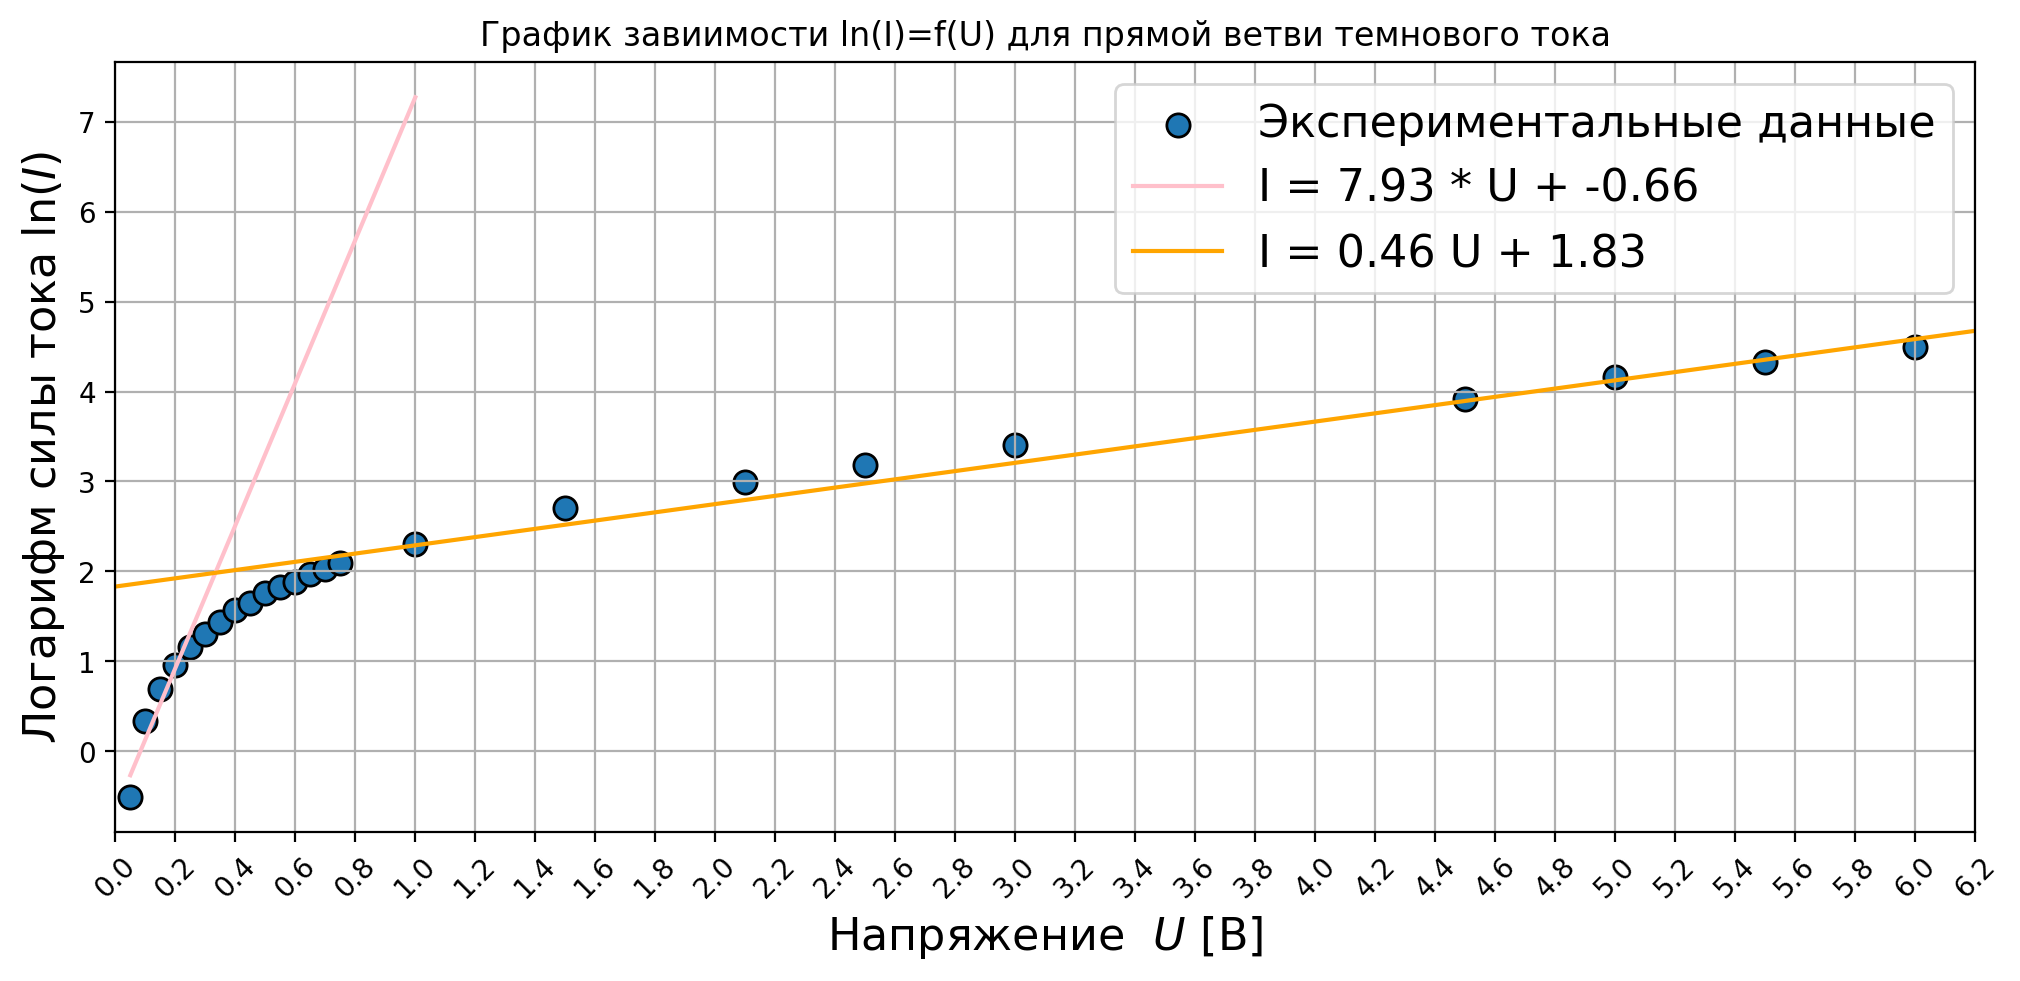
\includegraphics[width=0.8\textwidth]{pics/ln.png}
    \caption{График зависимости $\ln(I) = f(U)$ для прямой ветви темновой характеристики}
    \label{fig:ln}
\end{figure}


Для прямой ветви построим график зависимости $ln(I)$ от $U$(смотрите рисунок \ref{fig:ln}).
Коэффициент наклона линейного участка зависимости позволяет найти параметры $A$ и $I_{s}$.

$$
I_{s} = e^{b} \sim 6 \text{ мкА}
$$

$$
A = \frac{1}{0.025 a} \sim 85.1
$$

\subsection*{\textcolor{sub_header}{Световые характеристики}}


Результаты измерений световой характеристики представлены на рисунке \ref{fig:light_straight}. Найдём наилучшие параметры функции $y = A e^{(x - b) / c} + O$, приближающие экспериментальную зависимость. 


Найденный параметр $O$ - есть ток короткого замыкания $\to$ $I_{\text{к.з.}} = 14 \pm 0.2 \text{мА}$. 
ЭДС холостого хода находится из условия отсутствия тока в цепи. Решая уравнение $A e^{(U_{\text{x.x.}} - b) / c} + O = 0$, получаем:
\begin{equation}
    U_{\text{x.x.}} = c \operatorname{ln}(\frac{-O}{A}) + b = 6.3 \pm 0.2 \text{В}
    \label{uxx}
\end{equation}




\begin{figure}[!hbtp]
    \centering
    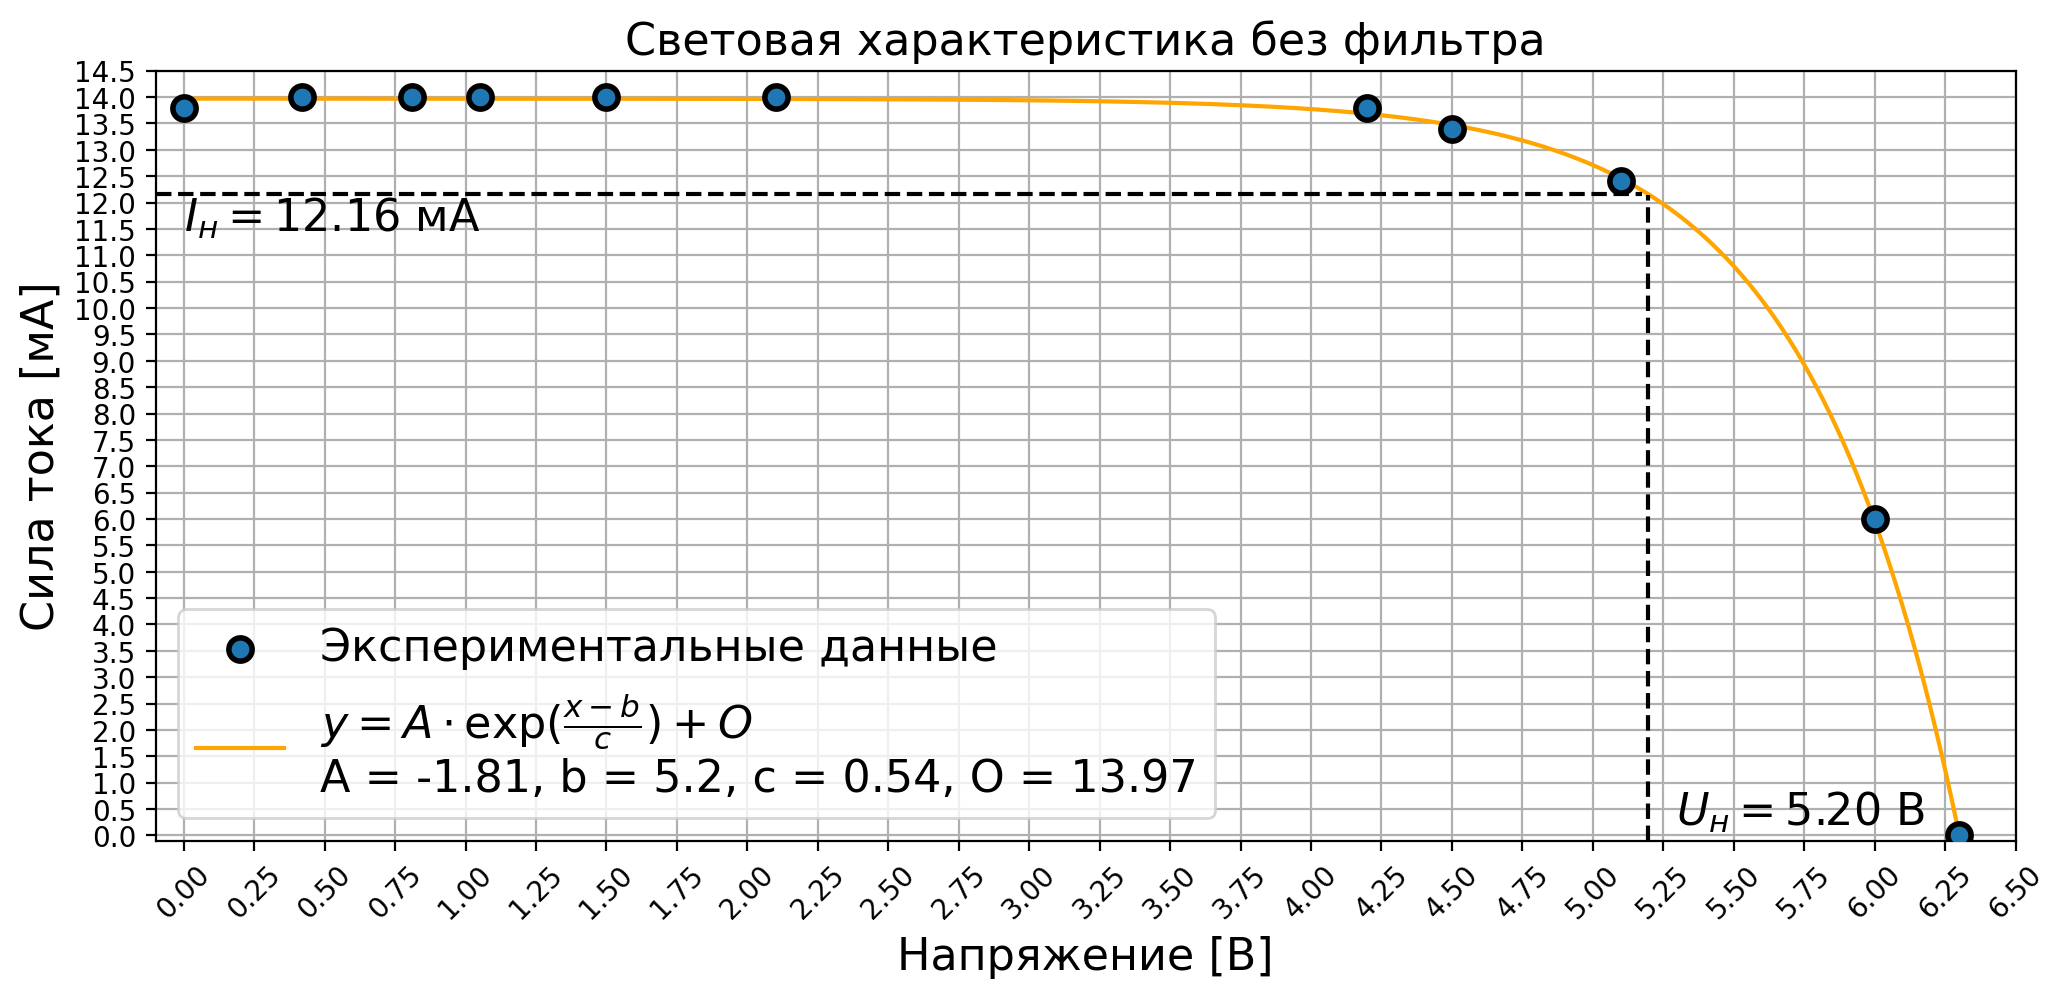
\includegraphics[width = 0.9\textwidth]{pics/no_filter.png}
    \caption{Зависимость $I = f(U)$ для световой характеристики.}
    \label{fig:light_straight}
\end{figure}


Параметр приближения $b$(точка излома) есть напряжение нагрузки $U_n = 5.2 \pm 0.1 \text{В}$.

Найдём силу тока нагрузки:
\begin{equation}
    I_{\text{н}} = A e^{(U_{\text{н}} - b) / c} + O = A + O =  12.2 \pm 0.2 \text{ мА}
    \label{in}
\end{equation}

Таким образом, сопротивление 
\begin{equation}
R_{\text{опт}} = \frac{U_{\text{н}}}{I_{\text{н}}} \sim 0.5 \text{ кОм}. 
\end{equation}


Найденные (см. формулы \ref{uxx}, \ref{in}) значения позволяют найти мощность преобразователя:
\begin{equation}
    P  = I_{\text{н}} U_{\text{н}} = 77 \pm 5 \text{ мВт}
\end{equation}

Оценим коэффициент заполнения нагрузочной характеристики:
\begin{equation}
    \xi = \frac{P}{U_{\text{х.х}} I_{\text{к.к}}} \sim 0.87
\end{equation}


Зная мощность падающего излучения $W = 550 \text{Вт}/\text{м}^{2}$ и площадь поверхности исследуемого образца $S \sim 100 \text{см}^2$ найдём КПД:
\begin{equation}
    \eta = \frac{P}{W S} \sim 0.01  
    \label{kpd}
\end{equation}



\subsection*{\textcolor{sub_header}{Световые характеристики снятые с использованием оптических фильтров}}



На рисунке \ref{fig:filters}, изображены ВАХ снятые при использовании оптических фильтров. Определим $I_{\text{к.з}}$ и $U_{\text{x.x.}}$ пользуясь описанной выше методикой:
$$
I_{\text{к.з.}}^{\text{красный}} \sim 11 \text{мА} \text{   } U_{\text{x.x}}^{\text{красный}} \sim 6.2 \text{В}
$$
$$
I_{\text{к.з.}}^{\text{темный}} \sim 6.93 \text{мА} \text{   } U_{\text{x.x}}^{\text{темный}} \sim 5.95 \text{В}
$$
\begin{figure}[htbp]
    \centering
    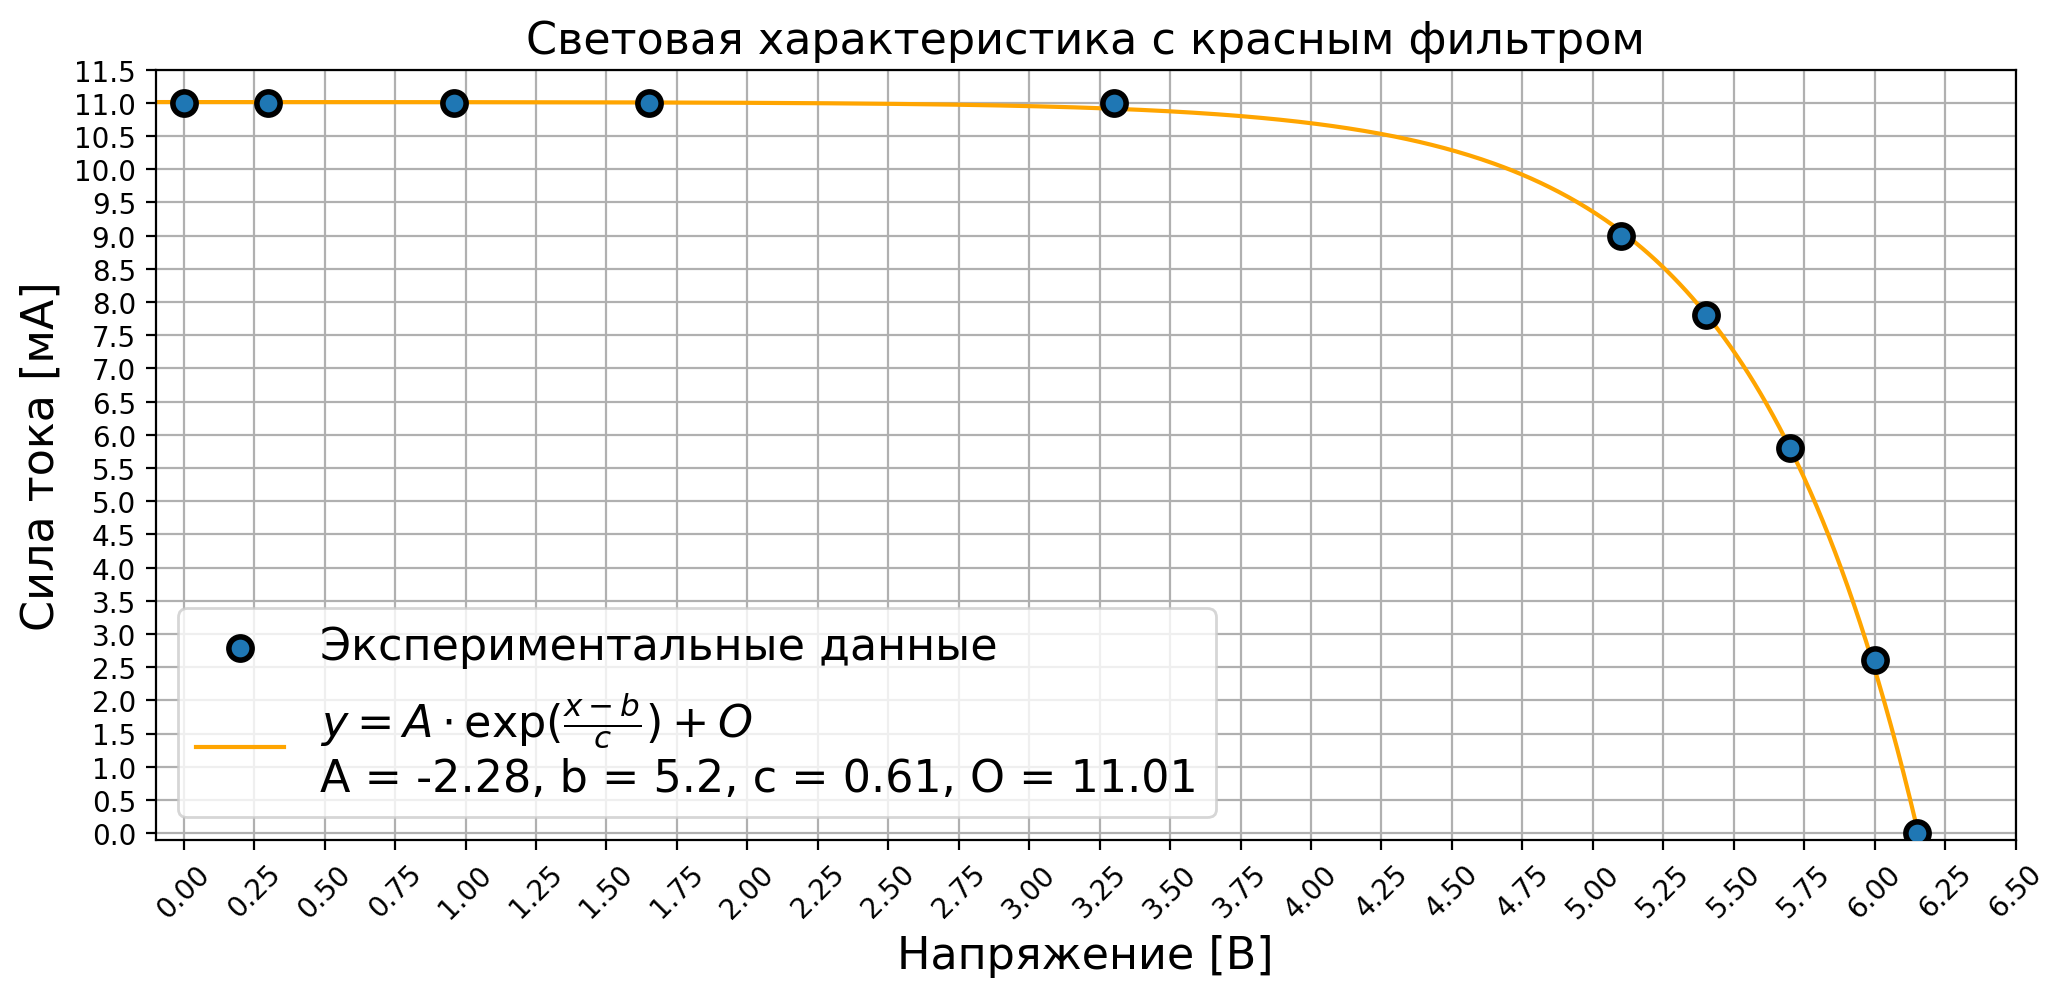
\includegraphics[width = 0.7\textwidth]{pics/red_filter.png} \hfill
    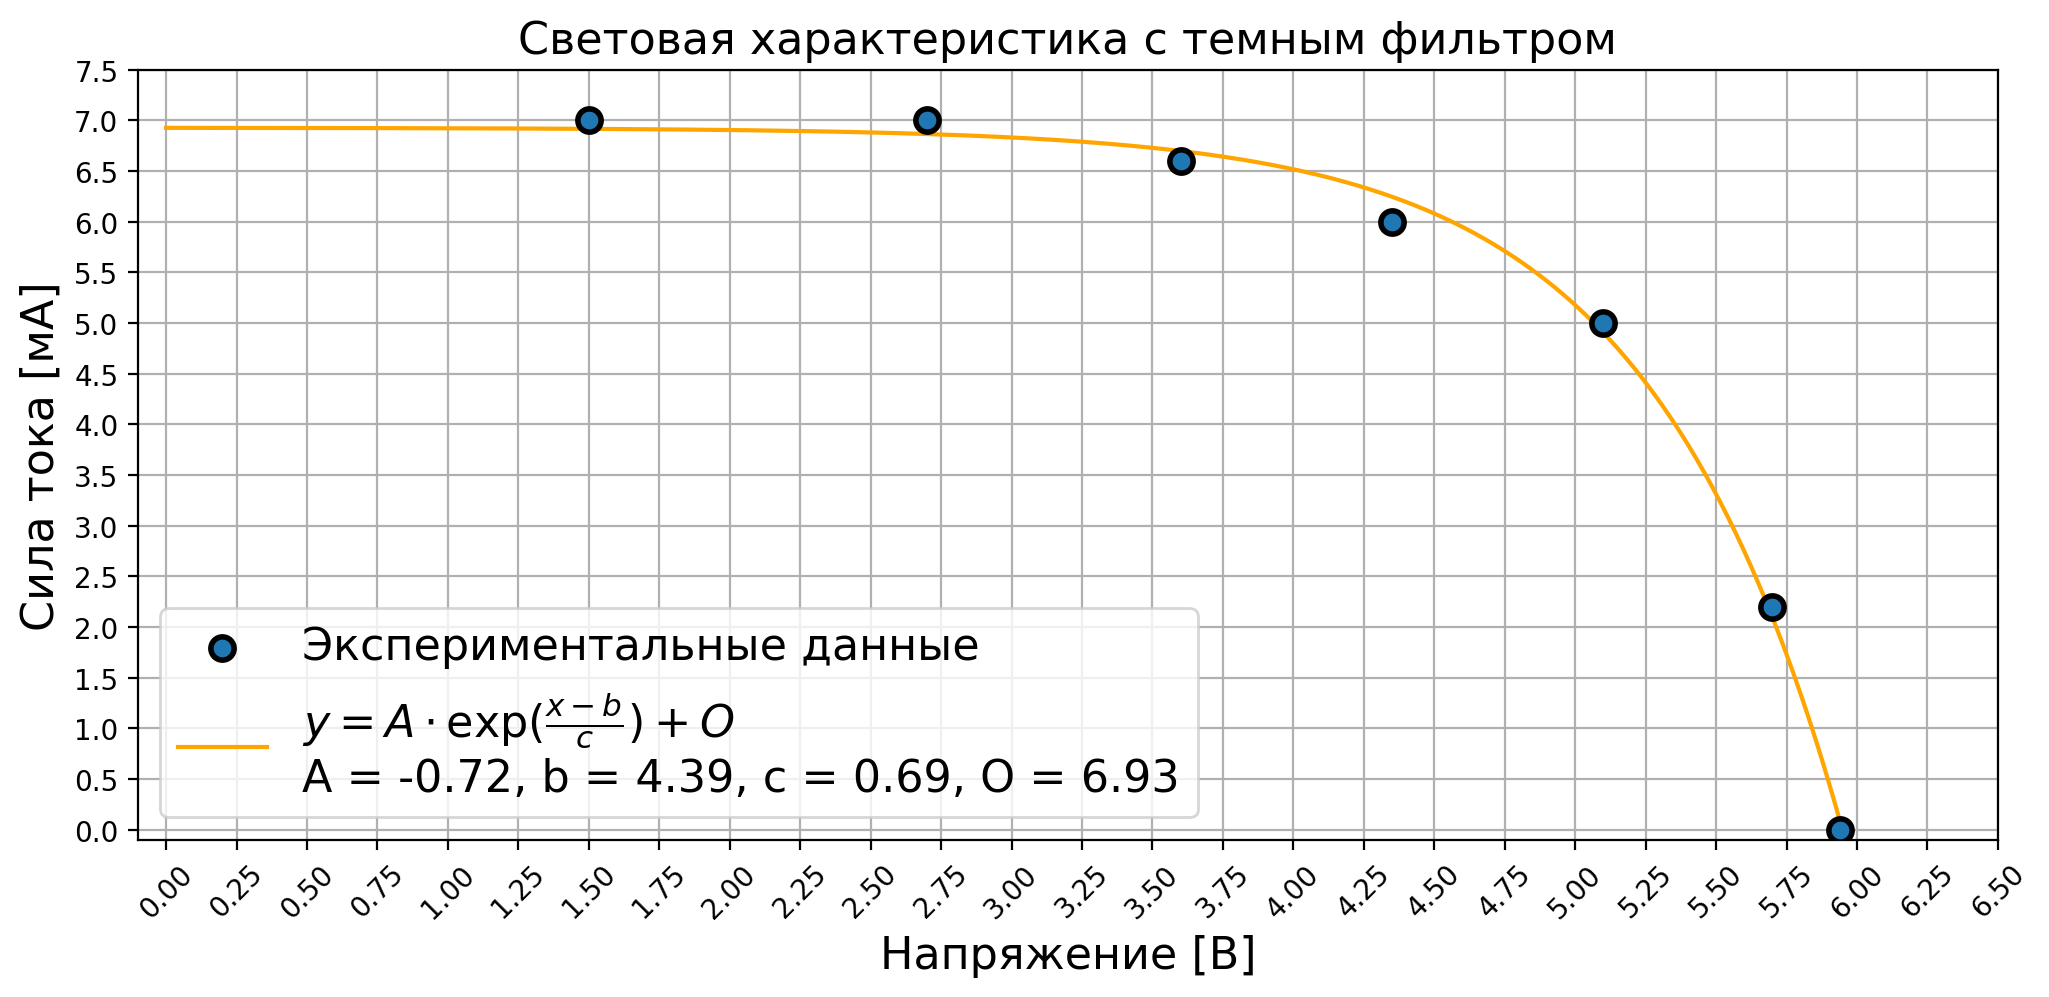
\includegraphics[width = 0.7\textwidth]{pics/black_filter.png}
    \caption{Зависимости $I = f(U)$ для световых характеристик, снятых при использовании красного и затемняющего фильтров.}
    \label{fig:filters}
\end{figure}


Построим график зависимости $ln(I_{\text{к.з.}})$ от $U_{x.x}$(смотрите рисунок \ref{fig:line}). Параметры прямой, проходящей через точки позволяют определить $I_s$.

\begin{equation}
    I_{s} = e^{b} \sim 0.05 \text{ мА}
\end{equation}

\begin{equation}
    A = \frac{1}{0.025 a} \sim 20
\end{equation}


\begin{figure}[htbp]
    \centering
    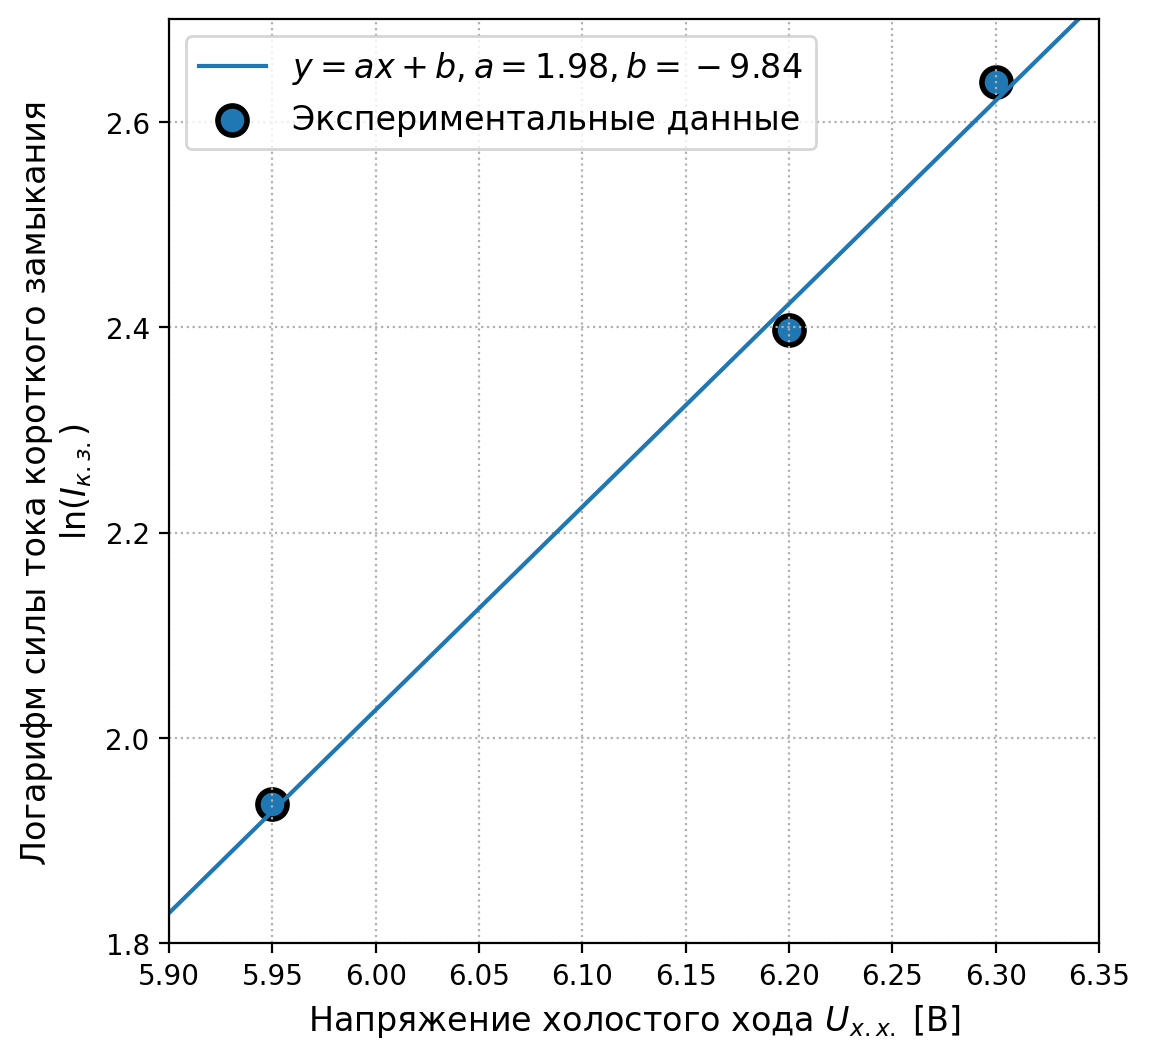
\includegraphics[width = 0.6\textwidth]{pics/line.png}
    \caption{Зависимость логарифма силы тока короткого замыкания от напряжения холостого хода}
    \label{fig:line}
\end{figure}

\newpage
\section*{\textcolor{header}{Вывод}}






\end{document}
